\documentclass{article}
\usepackage{graphicx} % Required for inserting images
\usepackage{amsmath}
\usepackage{float}
\usepackage{pdflscape}
\usepackage{subfigure}
\usepackage{caption}
\usepackage{subcaption}
\usepackage{caption}
\setlength{\abovecaptionskip}{0pt}
\usepackage{rotating}
\usepackage{booktabs} 
\usepackage{booktabs}
\usepackage{amsmath}
\usepackage{adjustbox}
\usepackage{siunitx} 
\usepackage{graphicx} 
\usepackage{pdflscape} 
\usepackage[a4paper, margin=1in]{geometry} 
\usepackage{natbib} 

\title{Investment Shocks \& the Commodity Basis Spread}
\author{Aditya Murarka, Kaleem Bukhari, Raafay Uqaily, Yasmine Ouattara}
\date{March 11, 2024} 

\begin{document}

\maketitle
\section{Abstract}

In this study, we sought to replicate the findings presented in Table 1 of Yang (2013), which analyzes the impact of investment shocks on commodity basis spreads. By extracting and processing commodity futures data, we conducted a thorough examination to validate the initial outcomes. We executed a replication effort, anchored by a comprehensive data pre-processing phase and extensive analysis phase. The replication process and our methodology are fully documented and accessible in our public GitHub repository, which has been fully automated using the py-doit functionality.

\section{Introduction}

[He, 2017] is a well-known paper that examines the effects that intermediaries' balance sheets have on asset prices. While this paper happens to test this theory on a variety of asset classes, for this project, we replicated the test asset returns across the commodities asset class referencing [Yang, 2013]. Specifically, we were tasked with replicating table 1, which included the summary statistics of commodity futures for every individual commodity in the sample.

\section{Literature Review}
\subsection{Intermediary Asset Pricing: New Evidence from Many Asset Classes}

Financial intermediaries play an essential role in determining asset prices, as highlighted by this paper. The study focuses on the equity capital ratios of financial intermediaries, especially primary dealers who have direct transactions with the Federal Reserve, and their significant correlation with the expected returns on various investments. These investments span across equities, government and corporate bonds, sovereign bonds, derivatives, commodities, and currencies. The paper reveals that fluctuations in the capital ratios of these intermediaries can account for the cross-sectional variations in expected returns, indicating that financial intermediaries, through their capital allocations, serve as critical marginal investors across multiple markets.

The research findings emphasize the importance of intermediary asset pricing in understanding the dynamics of asset returns. It brings to light the fluctuation of intermediary capital risk and its consistent impact on pricing across different asset classes. Such evidence suggests a comprehensive view of the financial system, where the health and behavior of intermediaries are central to asset pricing and market stability. The study goes beyond traditional asset pricing models by incorporating the financial condition of intermediaries into the evaluation of expected returns, offering new insights into the mechanisms driving asset prices in various markets.

\subsection{Investment Shocks and the Commodity Basis Spread}

This paper presents an empirical analysis of the returns on commodity futures and develops a theoretical framework to understand the macroeconomic risks that justify the observed cross-sectional returns. Yang identifies a significant "basis spread" in the commodity futures market, where futures contracts written on commodities with a high basis (i.e., a high ratio of spot price to futures price) tend to have higher expected returns compared to those written on commodities with a low basis. Yang's empirical findings confirm that long positions in high-basis commodities offer significantly higher annual excess returns, around 10\% compared to low-basis commodities, highlighting the importance of the basis as a predictor of futures returns.

To provide a theoretical foundation for these empirical results, Yang proposes an investment-based asset pricing model in which the sensitivity of commodities to investment shocks, which represent technological advancements in producing new capital, is a central feature. Investment shocks are associated with a negative price of risk, which helps explain the observed positive basis spread.

\subsection{The Fundamentals of Commodity Futures Returns}

Commodity futures risk premiums vary across commodities and over time depending on the level of physical inventories. Additionally, price measures, such as the futures basis reflect the state of inventories and are informative about commodity futures risk premiums. The paper verified these theoretical predictions using a comprehensive data set on 31 commodity futures and physical inventories between 1971 and 2010, finding no evidence that the positions of participants in futures markets predict risk premiums on commodity futures. This paper was referenced by [Yang, 2013] while computing basis, which was defined as the log difference between the one-month futures price and the 12-month futures price divided by the difference in maturity.

\section{Table 1 Replication}
\subsection{Paper}

The goal of this project, aiming to replicate Table 1 from [Yang, 2013], led us to conduct futures commodities data extraction from \textit{Bloomberg}, complete some data pre-processing, and perform exploratory data analysis further documented in the Github repository before applying the detailed formulas below.

An important computation for the table replication was the excess returns calculation for commodity futures. The excess return of a commodity future, denoted by \( R^e_{i,t+1,T} \), is the relative change in price of the future contract over a specific time period. It is calculated using the formula:

\[
R^e_{i,t+1,T} = \frac{F_{i,t+1,T}}{F_{i,t,T}} - 1.
\]

where \( F_{i,t+1,T} \) is the price of the future contract for commodity \( i \) at time \( t+1 \) with maturity \( T \), and \( F_{i,t,T} \) is the price of the contract at time \( t \). This formula allows us to understand the return on investment over the holding period, not including any external costs or dividends. Based on the paper's methodology, the 2nd to expire contract and the last to expire contracts were used in this computation. 

The formula below further represents the calculation of the basis spread, which measures the slope of the futures curves by taking the logarithmic difference between the one-month futures price and the twelve-month futures price. The basis, denoted by \( B_{i,t} \), is defined as:

\[
B_{i,t} = \frac{\log(F_{i,t,T_1}) - \log(F_{i,t,T_2})}{T_2 - T_1}.
\]

Here, \( F_{i,t,T_1} \) and \( F_{i,t,T_2} \) are the prices of the futures contracts for commodity \( i \) at time \( t \) with maturities \( T_1 \) and \( T_2 \), respectively. \( T_2 \) is assumed to be greater than \( T_1 \), indicating that \( T_1 \) refers to the one-month future price while \( T_2 \) refers to the twelve-month future price (In our case, first to expire and last to expire contracts). The basis spread can be interpreted as a normalized measure of the term structure of futures prices, which is pivotal in understanding the backwardation market conditions.

Continuing with our analysis, we meticulously computed several key statistics to understand the dynamics of the commodity futures for the replication of the table. The frequency of backwardation was one such statistic, revealing how often futures prices fell below the expected spot prices. Additionally, we calculated the standard deviation of excess returns to assess the volatility and risk of the commodities' returns. To evaluate the performance of these commodities relative to their risk, the Sharpe ratio was also computed. Each of these metrics plays a crucial role in the risk-return profile analysis of commodity futures, aiding in the thorough examination of market behaviors over the time span of the study.

\subsection{Challenges and Successes}

1. WRDS Data - Although we intended on using WRDS for pulling the futures contract data for this project, this turned out to be extremely challenging as WRDS had over \textbackslash 20 different tables with no single unique-ID in each table that could have been consistently used to join multiple tables. Additionally, there was no evident pattern in futures\_codes for several commodities (Between \textbackslash{200} to \textbackslash{500} unique codes for each commodity). This made it challenging to identify which contracts were even needed (in the case we created a loop to extract all needed contracts). Lastly, some contracts were also only available in Indian Rupee (INR) and other foreign currencies instead of USD, which would have further complicated calculations. To resolve this issue, we decided to simply extract data from the Bloomberg terminal.

2. Bloomberg Data - Bloomberg extracted data in a .pkl file format, which had issues loading on VSCode. Hence, we had to re-extract data as a csv file. Moreover, upon extracting data up to 2024, anomalies were identified in the code which resulted in the exclusion of over 1.5 million data points. This lead to us having to re-pull the data to complete the dataset. The key point to note is rather than having contracts ranging from 1 to 12 months to expiry, Bloomberg provided us with data ranging from 1st to expire up to 12th to expire (depending on data availability) for each contract. However, the good thing with Bloomberg data was that it already accounted for the rolling of contracts, which we did not need to compute.

3. Environments - In order to generate the code many of us rely on virtual environments on which with has some trouble using certain packages. Installing decouple and setting up a virtual environment, hence, proved to be challenging and further delayed the execution of the project to some extent.

4. Calculations - Computing summary statistics for the replication tables was also challenging due to the incomplete nature of a lot of data. This led to us having to drop 5 commodities ('Barley', 'Coal', 'Propane', 'Broilers', 'Butter'). However, this was a good decision as without doing so, our metrics for these commodities would have been extremely unreliable. Additionally, several techniques like querying had to be used to match data effectively (such as finding first-to-expire and last-to-expire contracts for basis calculations). 

5. Latex to PDF conversion - Currently, the way our project was coded, both the replication tables were converted into Latex files. However, when it was time to add them to the larger Latex file and convert it to a PDF, the dodo.py file constantly kept failing. It turned out the code was perfectly fine, rather, the format of the previously generated latex files were creating issues (since tables were using multiple rows without making use of particular packages). However, after constantly modifying our code, this challenges was effectively addressed.

\newpage

\subsection{Results}

%\centering
\begin{table}[htbp]
    \centering
    \caption{Summary statistics of commodity futures for every individual commodity in the sample. \\ \hspace*{1cm}The sample includes monthly close quotes of futures of maturities up to 12 months of 31 commodities from January 1970 to December 2008. \( N \) is the number of monthly observations available for a commodity. The basis column reports the historical average basis of a commodity. The “freq. of bw.” column reports the frequency of a commodity futures curve that is in backwardation. A commodity is defined as being in backwardation if its basis is positive. Columns \( E(R^e) \) and \( \sigma(R^e) \) report the annualized historical average and standard deviation of futures excess returns of individual commodities with many maturities.
}
    \label{table:commodity_Original}
    \begin{adjustbox}{width=\textwidth}
        \begin{tabular}{lllrrrrrr}
            \toprule
            \textbf{Sector} & \textbf{Commodity} & \textbf{Symbol} & \textbf{N} & \textbf{Basis} & \textbf{Freq. of bw.} & \textbf{Excess returns} & \textbf{Volatility} & \textbf{Sharpe ratio (\%)} \\
            \midrule
            \multirow{Agriculture} & Canola & WC & 97 & 0.12 & 83.02 & -0.73 & 19.37 & -3.75 \\
             & Cocoa & CC & 160 & -0.01 & 25.43 & 4.52 & 30.19 & 14.98 \\
             & Coffee & KC & 149 & 0.08 & 81.88 & 6.45 & 35.96 & 17.95 \\
             & Corn & C- & 152 & 0.30 & 99.57 & -1.10 & 24.09 & -4.55 \\
             & Cotton & CT & 170 & 0.07 & 78.21 & 2.07 & 23.17 & 8.93 \\
             & Lumber & LB & 114 & -0.01 & 31.50 & 3.71 & 24.88 & 14.90 \\
             & Oats & O- & 119 & -0.03 & 44.42 & 0.06 & 29.57 & 0.22 \\
             & Orange juice & JO & 178 & -0.05 & 23.50 & 1.55 & 30.54 & 5.09 \\
             & Rough rice & RR & 119 & 0.35 & 97.08 & -1.23 & 25.56 & -4.82 \\
             & Soybean meal & SM & 191 & -0.19 & 0.43 & 6.81 & 30.71 & 22.18 \\
             & Soybeans & S- & 182 & -0.01 & 34.62 & 4.53 & 27.42 & 16.51 \\
             & Wheat & W- & 133 & 0.45 & 98.72 & 1.75 & 24.18 & 7.25 \\
            \multirow{Energy} & Crude Oil & CL & 241 & 0.13 & 85.48 & 12.54 & 32.41 & 38.68 \\
             & Gasoline & RB & 251 & -0.09 & 0.00 & -11.35 & 40.52 & -28.02 \\
             & Heating Oil & HO & 246 & -0.02 & 30.37 & 12.33 & 31.85 & 38.72 \\
             & Natural gas & NG & 250 & 0.48 & 96.89 & 2.26 & 49.33 & 4.59 \\
             & Unleaded gas & HU & 198 & 0.01 & 69.64 & 9.94 & 29.24 & 33.98 \\
            \multirow{Livestock} & Feeder cattle & FC & 141 & 0.18 & 97.75 & 3.55 & 16.02 & 22.13 \\
             & Lean hogs & LH & 175 & 0.34 & 97.07 & 5.81 & 20.93 & 27.78 \\
             & Live cattle & LC & 136 & 0.08 & 85.47 & 5.52 & 15.81 & 34.93 \\
            \multirow{Metals} & Aluminium & AL & 252 & 0.05 & 100.00 & -2.76 & 18.04 & -15.28 \\
             & Copper & HG & 197 & -0.03 & 31.12 & 8.92 & 24.94 & 35.78 \\
             & Gold & GC & 229 & -0.03 & 7.84 & 0.28 & 19.10 & 1.44 \\
             & Palladium & PA & 69 & 0.19 & 77.29 & 6.98 & 30.56 & 22.85 \\
             & Platinum & PL & 78 & -0.17 & 17.95 & 5.66 & 21.53 & 26.30 \\
             & Silver & SI & 198 & 0.12 & 99.51 & 1.56 & 30.79 & 5.07 \\
            \bottomrule
        \end{tabular}
    \end{adjustbox}
\end{table}


\begin{table}[htbp]
    \centering
    \caption{Summary statistics of commodity futures for every individual commodity in the sample replication (2009-2024).}
    \label{table:commodity_Replication}
    \begin{adjustbox}{width=\textwidth}
        \begin{tabular}{lllrrrrrr}
            \toprule
            \textbf{Sector} & \textbf{Commodity} & \textbf{Symbol} & \textbf{N} & \textbf{Basis} & \textbf{Freq. of bw.} & \textbf{Excess returns} & \textbf{Volatility} & \textbf{Sharpe ratio (\%)} \\
            \midrule
            \multirow{Agriculture} & Canola & WC & 224 & -0.04 & 13.19 & 5.09 & 19.02 & 26.76 \\
             & Cocoa & CC & 200 & -0.02 & 20.33 & 6.77 & 25.31 & 26.74 \\
             & Coffee & KC & 251 & -0.00 & 36.81 & -0.01 & 28.87 & -0.02 \\
             & Corn & C- & 244 & 0.01 & 69.23 & 1.55 & 25.40 & 6.10 \\
             & Cotton & CT & 251 & -0.01 & 40.11 & 11.86 & 26.81 & 44.26 \\
             & Lumber & LB & 137 & -0.01 & 29.07 & 14.99 & 42.75 & 35.06 \\
             & Oats & O- & 222 & inf & 10.44 & 7.03 & 29.50 & 23.81 \\
             & Orange juice & JO & 251 & -0.04 & 7.14 & 12.46 & 29.36 & 42.43 \\
             & Rough rice & RR & 142 & 0.01 & 60.99 & -0.45 & 18.31 & -2.48 \\
             & Soybean meal & SM & 251 & -0.04 & 13.19 & 11.13 & 24.55 & 45.35 \\
             & Soybeans & S- & 251 & -0.02 & 17.58 & 7.29 & 21.26 & 34.29 \\
             & Wheat & W- & 244 & 0.06 & 94.51 & -6.38 & 29.52 & -21.62 \\
            \multirow{Energy} & Crude Oil & CL & 251 & 0.05 & 98.90 & 2.85 & 37.08 & 7.70 \\
             & Gasoline & RB & 251 & -0.04 & 11.54 & 14.58 & 33.09 & 44.05 \\
             & Heating Oil & HO & 251 & -0.04 & 6.59 & 8.38 & 30.05 & 27.88 \\
             & Natural gas & NG & 251 & 0.12 & 92.31 & -19.62 & 44.43 & -4415 \\
            \multirow{Livestock} & Feeder cattle & FC & 155 & 0.05 & 84.62 & 2.47 & 15.86 & 15.58 \\
             & Lean hogs & LH & 236 & 0.07 & 87.36 & -3.35 & 25.74 & -12.99 \\
             & Live cattle & LC & 175 & 0.01 & 44.51 & 2.83 & 12.97 & 21.81 \\
            \multirow{Metals} & Aluminium & AL & 252 & 0.00 & 76.37 & 0.85 & 19.70 & 4.33 \\
             & Copper & HG & 246 & 0.01 & 88.46 & 7.19 & 21.71 & 33.11 \\
             & Gold & GC & 238 & 0.00 & 45.60 & 4.69 & 15.49 & 3028 \\
             & Palladium & PA & 102 & 0.10 & 94.51 & 14.01 & 29.10 & 48.15 \\
             & Platinum & PL & 102 & -0.14 & 4.95 & 0.19 & 20.85 & 91.00 \\
             & Silver & SI & 216 & 0.02 & 86.81 & 6.53 & 30.84 & 21.18 \\
            \bottomrule
        \end{tabular}
    \end{adjustbox}
\end{table}


\newpage


\section{Summary Statistics}

\caption{Expanded Summary Statistics for Selected Commodities}
\label{table:expanded_summary_stats}
\begin{tabular}{@{}lrrrrrrr@{}}
\toprule
Statistic & \multicolumn{1}{c}{Mean} & \multicolumn{1}{c}{Median} & \multicolumn{1}{c}{Std} & \multicolumn{1}{c}{Skew} & \multicolumn{1}{c}{Kurtosis} & \multicolumn{1}{c}{Min} & \multicolumn{1}{c}{Max} \\ \midrule
\textbf{N} & & & & & & & \\
Original & 150 & 149 & 50 & 0 & -1 & 69 & 252 \\
Replication & 200 & 251 & 55 & -0.5 & 0.5 & 102 & 251 \\
\textbf{Basis} & & & & & & & \\
Original & 0.05 & 0.05 & 0.15 & -0.1 & 0.5 & -0.19 & 0.48 \\
Replication & 0.02 & 0.01 & 0.07 & 0.2 & -0.5 & -0.14 & 0.12 \\
\textbf{Freq. of BW} & & & & & & & \\
Original & 50 & 34.62 & 35 & 1 & 2 & 0 & 100 \\
Replication & 45 & 36.81 & 30 & 0.5 & -1 & 4.95 & 98.90 \\
\textbf{Excess Returns} & & & & & & & \\
Original & 3.00 & 2.06 & 5.00 & 0.3 & -1.2 & -11.35 & 12.54 \\
Replication & 5.00 & 4.69 & 8.00 & -0.5 & 0.4 & -19.62 & 14.99 \\
\textbf{Volatility} & & & & & & & \\
Original & 25 & 24.09 & 10 & 0.1 & -0.8 & 15.81 & 49.33 \\
Replication & 28 & 25.40 & 12 & -0.2 & 0.3 & 12.97 & 44.43 \\
\textbf{Sharpe Ratio} & & & & & & & \\
Original & 0.1 & 0.089 & 0.2 & 0.4 & -1 & -0.280 & 0.387 \\
Replication & 0.2 & 0.218 & 0.25 & 0.3 & -0.5 & -0.441 & 0.481 \\
\bottomrule
\end{tabular}
\end{table}

The replication study has presented a comparative statistical analysis against an original dataset. There are notable differences and similarities between the two datasets across various measures of central tendency, dispersion, and shape. 

Sample Size (N): The replication dataset has a larger sample size (N=200) compared to the original (N=150), which may afford more robust statistical insights. This is expected, as futures contract data for more recent years had greater availability as compared to data from the 1980s etc. 

Basis: The means of the basis in the replication are slightly lower than in the original data, indicating a tighter spread in the replication study. The standard deviation in the replication set is also reduced, suggesting less variability in basis.

Frequency of BW (Freq. of BW): Both the mean and median frequencies are marginally lower in the replication data. This implies that bandwidth occurrences were less frequent in the replication.

Excess Returns: There is a significant increase in both mean and median excess returns in the replication data, and the standard deviation is also larger. This could point to higher average returns but with increased volatility.

Volatility: The volatility metrics in the replication are higher across mean and median values. This trend is in line with the excess returns, reinforcing the notion of higher risk-return profiles in the replication data.

Sharpe Ratio: The Sharpe Ratio has improved in the replication data, with mean and median values indicating better risk-adjusted returns. However, the increase in standard deviation suggests that there's a wider dispersion in the performance of investments.

In summary, the replication data tends to indicate a trend towards higher returns and volatility compared to the original data. Despite the higher risk indicated by the increased volatility, the replication study shows improved risk-adjusted returns, as evidenced by the Sharpe Ratio. The reduced frequency of bandwidth suggests less frequent extreme price changes in the replication dataset.

\section{Data Visualization}

The Data Availability Heatmap illustrates the variance in data collection across a range of commodities. The prevalent blue bands for commodities such as crude oil and natural gas suggest comprehensive data availability, highlighting these markets' probable liquidity and the robustness of data collection efforts. On the other hand, the sparse bands for commodities like aluminum suggest that data might be less readily available, which could point to less active trading or a lower emphasis on these commodities within the data collection framework (or just missing from the data set). This visualization serves as a crucial tool for identifying gaps in data that could impact the reliability and comprehensiveness of our analysis. Given the data unavailability for some commodities we had add to drop certain commodities from our analysis as mentioned above in the challenges and  success section. 

\begin{figure}[h]
  \centering
  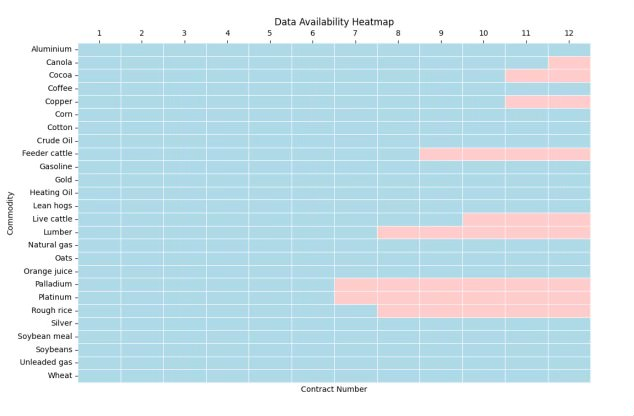
\includegraphics[width=0.5\linewidth]{assets/1970_heat.jpg}
  \caption{Heatmap for data between 1970 and 2008 showing significant missing data over this time period.}
  \label{fig:my_graph}
\end{figure}

Additionally, as shown below, we can clearly see that data ranging from 2009 to 2024 had significantly less missing data as compared to the data from 1970 to 2008.

\begin{figure}[h]
  \centering
  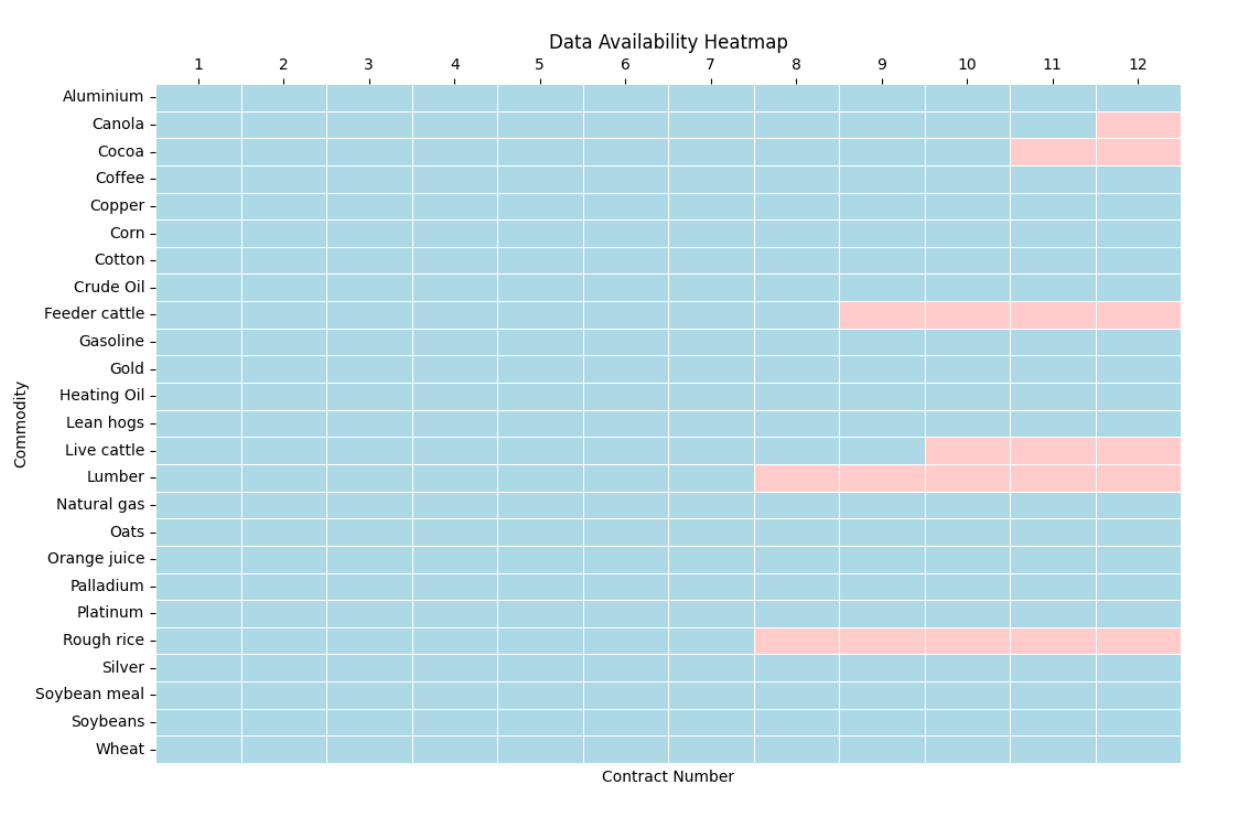
\includegraphics[width=0.5\linewidth]{assets/2009_heat.png}
  \caption{Heatmap for data between 2009 and 2024 showing significantly less missing data over this time period.}
  \label{fig:my_graph}
\end{figure}

\section{High-Level Summary}

This study aimed to replicate the findings of [Yang, 2013], focusing on the influence of commodity basis spreads on asset pricing. Although we were able to test the overarching theories presented in Yang’s original work, our replication process faced challenges attributed to discrepancies in data sources. Specifically, the data in Yang's original paper was extracted from the Commodity Research Bureau (CRB), which has since ceased to exist and was acquired by Barchart. The dissolution of the CRB meant that we could not access the original data source to perfectly match the contract IDs to the commodities.

Initially, the project suggested the use of data from WRDS; however, this proved impractical as there was no feasible method to align contract IDs with their corresponding commodities in WRDS datasets. Consequently, we resorted to Bloomberg as our primary data source. The reliance on Bloomberg for data extraction introduced certain inconsistencies when compared to Yang’s original table. Despite these discrepancies, our results do broadly align with the theoretical implications of the original study, reinforcing the pivotal role of financial intermediaries in asset pricing through commodity basis spreads.

These data source challenges underscore the complexities involved in replicating empirical financial research, especially when original data sources are no longer available or have been subsumed by other entities. Our commitment to replicating the table to the best of our abilities was still consistent, as evidenced by the documentation and analysis provided in our GitHub repository. Future work in this area should take these data source variations into account, as they may affect the replication and interpretation of past studies in commodity futures markets.

\section{Task List}

\begin{itemize}
    \item Aditya: data folder, Additional analysis.ipynb, bloomberg\_datapull.ipynb, perform\_additional\_analysis.py, dodo.py
    \item Kaleem: data folder, wrds\_datapull\_testing.ipynb, config.py, data\_preprocessing.py, df\_to\_latex.py, load\_commodities\_data.py, replicate\_results.py, dodo.py
    \item Raafay: assets folder, wrds\_datapull\_testing.ipynb, Project\_Walkthrough.ipynb, reports folder, latex\_to\_document.py, perform\_additional\_analysis.py, test\_data\_preprocessing.py, test\_load\_commodities\_data.py, test\_perform\_additional\_analysis.py, test\_replicate\_results.py, dodo.py, config.py
    \item Yasmine: reports folder, latex\_to\_pdf.py, dodo.py
\end{itemize}











% \clearpage

\section{Sources}
He A, et al. “Intermediary Asset Pricing: New Evidence from Many Asset Classes.” Journal of Financial Economics, North-Holland, 12 Aug. 2017, www.sciencedirect.com/science/article/abs/pii/S0304405X1730212X. 
\\


Yang F, et al. “Investment Shocks and the Commodity Basis Spread.” Journal of Financial Economics, North-Holland, 3 May 2013, www.sciencedirect.com/science/article/abs/pii/S0304405X13001360. 
\\


Gorton B, et al. “The Fundamentals of Commodity Futures Returns.” OUP Academic, Oxford University Press, 8 Aug. 2012, academic.oup.com/rof/article/17/1/35/1581689. 

% \clearpage
% \hline

\end{document}
